% ====================================================================
%  Chapter: Multi-User Behavior Learning & Personalization
% ====================================================================
\newpage
\section{Multi-User Behavior Learning \& Personalization Pipeline}
\label{sec:personalization}

While the HERA multi-agent system provides intelligent natural language
understanding and device control, it currently treats all household
members identically. Every user receives the same responses, follows the
same automation rules, and shares a single set of environmental
preferences. This chapter introduces a machine learning pipeline that
learns individual user behaviors, predicts personal preferences, and
enables truly personalized smart home experiences without requiring
explicit configuration from users.

\subsection{Why Personalization Requires Machine Learning}

\subsubsection{Limitations of rule-based approaches}

Traditional smart home systems rely on if-then rules or configurable
thresholds. While simple to implement, this approach fails to capture
the nuanced nature of human behavior:
\begin{itemize}
    \item \textbf{Context dependency:} The same action (e.g., turning on
    lights) may be preferred at different brightness levels depending on
    time of day, current activity, or ambient conditions.
    \item \textbf{Individual differences:} Family members have different
    comfort zones, sleep schedules, and device usage patterns that cannot
    be captured by shared global rules.
    \item \textbf{Temporal patterns:} User preferences follow complex
    weekly rhythms (weekday vs weekend), seasonal variations, and evolving
    habits that rigid rules cannot model.
    \item \textbf{Implicit preferences:} Users rarely explicitly configure
    their preferences, but their historical actions reveal clear patterns.
\end{itemize}

\subsubsection{The case for learned behavior models}

Machine learning addresses these limitations by automatically discovering
patterns from historical user interactions. Instead of requiring users to
manually configure hundreds of rules, the system observes natural
behavior and builds personalized models that predict:
\begin{itemize}
    \item What devices a user is likely to control given current context;
    \item Preferred device states (brightness, temperature setpoints);
    \item Optimal timing for proactive suggestions;
    \item Context-specific preferences (work mode vs relaxation mode).
\end{itemize}

This approach transforms the smart home from a passive rule executor into
an adaptive assistant that learns each household member's unique
preferences.

\subsubsection{System boundary: where rules end and learning begins}

Table~\ref{tab:rule-ml-boundary} clarifies the architectural separation
between deterministic rules and learned personalization.

\begin{table}[H]
    \centering
    \caption{Separation of concerns between rule-based and ML-based systems.}
    \label{tab:rule-ml-boundary}
    \renewcommand{\arraystretch}{1.2}
    \small
    \begin{tabularx}{\textwidth}{@{} >{\raggedright\arraybackslash}p{3cm} X X @{}}
        \toprule
        \textbf{Component} & \textbf{Responsibility} & \textbf{Rationale} \\
        \midrule
        Rule-based threshold system &
        Safety bounds (temperature limits, humidity alerts), hard automation triggers, and user-configurable constraints. &
        Safety-critical decisions must be deterministic, auditable, and immediately adjustable without retraining. \\
        ML personalization pipeline &
        Learning individual user patterns, predicting preferred actions and device states, generating context-aware suggestions. &
        Personal preferences are implicit, context-dependent, and vary by individual—precisely where learning provides value. \\
        HERA LLM agents &
        Natural language understanding, command execution, explanation generation, and conflict mediation. &
        LLM handles flexible language input/output while ML provides behavioral intelligence. \\
        \bottomrule
    \end{tabularx}
\end{table}

This separation ensures that safety-critical functionality remains
transparent and controllable, while personalization leverages the
pattern-learning strengths of machine learning.

\subsection{System Architecture Overview}
\label{sec:personalization-architecture}

Figure~\ref{fig:personalization-architecture} illustrates the complete
multi-user personalization architecture and its integration with the
existing HERA system.

\begin{figure}[H]
    \centering
    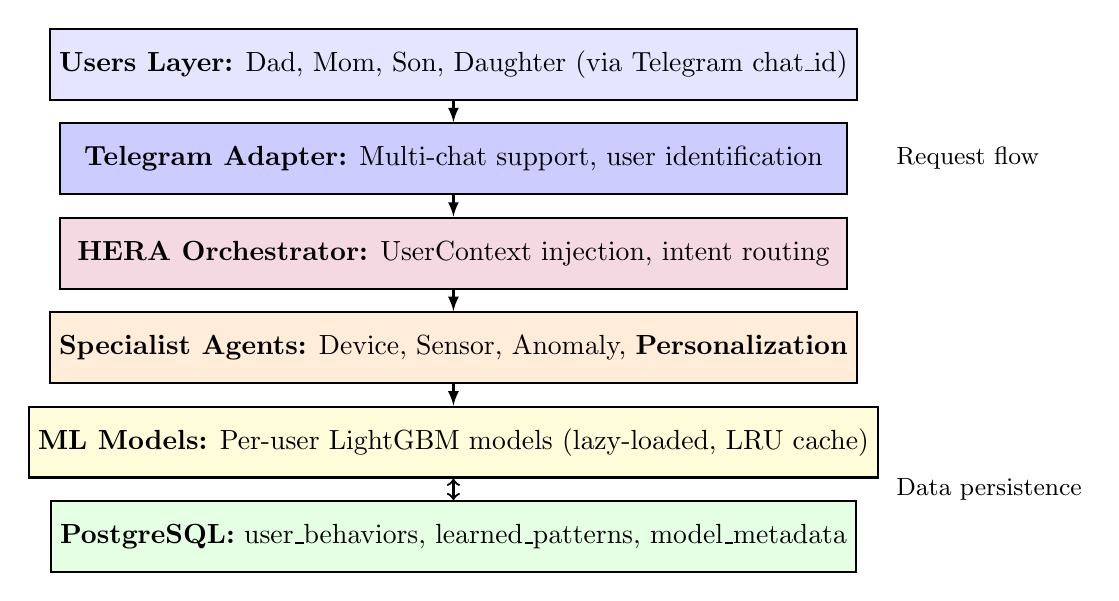
\begin{tikzpicture}[
        node distance=0.8cm,
        layer/.style={rectangle, draw, thick, minimum width=10cm, minimum height=0.9cm, align=center},
        arrow/.style={-latex, thick}
    ]
        % Vertical stack - simple layers
        \node[layer, fill=blue!10] (users) at (0, 6) {\textbf{Users Layer:} Dad, Mom, Son, Daughter (via Telegram chat\_id)};
        
        \node[layer, fill=blue!20] (telegram) at (0, 4.8) {\textbf{Telegram Adapter:} Multi-chat support, user identification};
        
        \node[layer, fill=purple!15] (orchestrator) at (0, 3.6) {\textbf{HERA Orchestrator:} UserContext injection, intent routing};
        
        \node[layer, fill=orange!15] (agents) at (0, 2.4) {\textbf{Specialist Agents:} Device, Sensor, Anomaly, \textbf{Personalization}};
        
        \node[layer, fill=yellow!15] (ml) at (0, 1.2) {\textbf{ML Models:} Per-user LightGBM models (lazy-loaded, LRU cache)};
        
        \node[layer, fill=green!10] (db) at (0, 0) {\textbf{PostgreSQL:} user\_behaviors, learned\_patterns, model\_metadata};
        
        % Simple vertical arrows
        \draw[arrow] (users) -- (telegram);
        \draw[arrow] (telegram) -- (orchestrator);
        \draw[arrow] (orchestrator) -- (agents);
        \draw[arrow] (agents) -- (ml);
        \draw[arrow, <->] (ml) -- (db);
        
        % Side annotation
        \node[align=left, font=\small, anchor=west] at (5.5, 4.8) {Request flow};
        \node[align=left, font=\small, anchor=west] at (5.5, 0.6) {Data persistence};
        
    \end{tikzpicture}
    \caption{Layered architecture of the multi-user personalization system. Each layer represents a distinct responsibility, from user identification through ML inference to data persistence.}
    \label{fig:personalization-architecture}
\end{figure}

\subsubsection{Key architectural components}

\paragraph{UserContext Injection Layer}
Every incoming message from Telegram includes a \texttt{chat\_id}
identifying the user. The orchestrator uses this to construct a
\texttt{UserContext} object containing:
\begin{itemize}
    \item User identity and role (admin, member, guest);
    \item Historical action patterns loaded from database;
    \item Current environmental context (sensor states, time of day);
    \item Learned preferences and conflict resolution priorities.
\end{itemize}

This context is injected into the system prompt of every specialist agent,
enabling personalized responses without requiring separate agent instances
per user.

\paragraph{Personalization Agent}
A new specialist agent responsible for:
\begin{itemize}
    \item Loading the appropriate per-user ML model (lazy loading with LRU cache);
    \item Predicting likely next actions given current context;
    \item Generating proactive suggestions when confidence exceeds threshold;
    \item Formatting predictions into natural language via LLM.
\end{itemize}

\paragraph{Per-User ML Models}
Rather than a single shared model, each household member has an individual
behavior model. This design choice optimizes for family-scale deployments
(3--5 users) where:
\begin{itemize}
    \item Individual models provide superior personalization;
    \item Memory overhead is acceptable (models are small and lazy-loaded);
    \item Model updates for one user don't affect others;
    \item Family members have genuinely different behavioral patterns.
\end{itemize}

For larger-scale deployments ($>$20 users), a shared model with user
embeddings (Netflix-style) would be more appropriate, but this is beyond
the scope of a family smart home system.

\paragraph{Asynchronous Behavior Logging}
Every user action is logged asynchronously to PostgreSQL without blocking
the response path. This ensures that personalization does not introduce
latency into the conversational interface. The logging pipeline captures:
\begin{itemize}
    \item Timestamp and user identifier;
    \item Device and action (e.g., \texttt{living\_room\_light: turn\_on, brightness=70});
    \item Environmental context at the time of action;
    \item Command success/failure status.
\end{itemize}

\paragraph{Conflict Resolution Engine}
When multiple users issue competing commands within a short time window,
the system applies a hierarchy of resolution strategies:
\begin{enumerate}
    \item \textbf{Role-based priority:} Admin $>$ Member $>$ Guest;
    \item \textbf{Temporal priority:} Most recent command wins if issued
    within 30-second window;
    \item \textbf{Negotiated compromise:} For continuous controls
    (brightness, temperature), compute weighted average based on user
    priorities;
    \item \textbf{LLM-mediated resolution:} In complex cases, orchestrator
    asks LLM to generate a natural language mediation message and propose
    compromise.
\end{enumerate}

\subsection{Data Pipeline and Feature Engineering}
\label{sec:data-pipeline}

Figure~\ref{fig:data-pipeline} shows the complete data flow from user
actions to trained personalization models.

\begin{figure}[H]
    \centering
    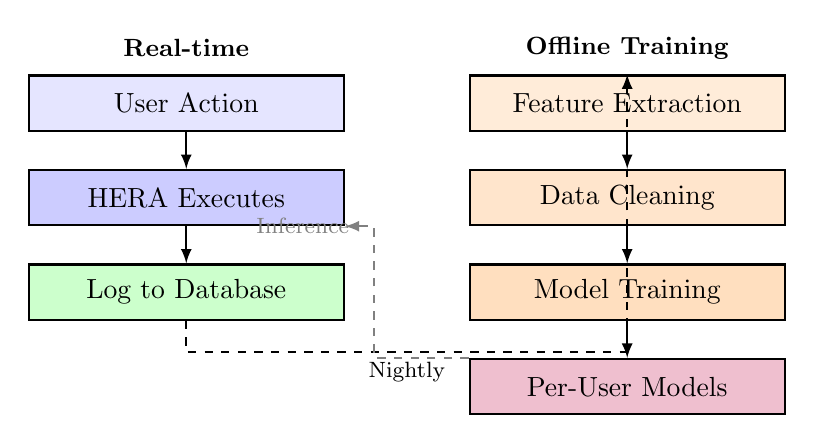
\begin{tikzpicture}[
        node distance=0.8cm,
        box/.style={rectangle, draw, thick, minimum width=4cm, minimum height=0.7cm, align=center},
        arrow/.style={-latex, thick}
    ]
        % Left column: Real-time flow (top to bottom)
        \node[box, fill=blue!10] (input) at (-2.8, 4.5) {User Action};
        \node[box, fill=blue!20] (hera) at (-2.8, 3.3) {HERA Executes};
        \node[box, fill=green!20] (log) at (-2.8, 2.1) {Log to Database};
        
        % Right column: Training pipeline (top to bottom)
        \node[box, fill=orange!15] (extract) at (2.8, 4.5) {Feature Extraction};
        \node[box, fill=orange!20] (clean) at (2.8, 3.3) {Data Cleaning};
        \node[box, fill=orange!25] (train) at (2.8, 2.1) {Model Training};
        \node[box, fill=purple!25] (models) at (2.8, 0.9) {Per-User Models};
        
        % Left column arrows
        \draw[arrow] (input) -- (hera);
        \draw[arrow] (hera) -- (log);
        
        % Right column arrows
        \draw[arrow] (extract) -- (clean);
        \draw[arrow] (clean) -- (train);
        \draw[arrow] (train) -- (models);
        
        % Cross arrows
        \draw[arrow, dashed] (log.south) -- ++(0,-0.4) -| (extract.north) 
            node[pos=0.25, below, font=\footnotesize] {Nightly};
        \draw[arrow, dashed, gray] (models.north west) -- ++(-1.2,0) |- (hera.south east)
            node[pos=0.75, left, font=\footnotesize] {Inference};
        
        % Column headers
        \node[font=\small\bfseries] at (-2.8, 5.2) {Real-time};
        \node[font=\small\bfseries] at (2.8, 5.2) {Offline Training};
        
    \end{tikzpicture}
    \caption{Two-phase data pipeline: real-time logging feeds offline training, models are hot-reloaded for inference.}
    \label{fig:data-pipeline}
\end{figure}

\subsubsection{Feature engineering strategy}

The model input consists of three feature groups:

\paragraph{Temporal features}
\begin{itemize}
    \item Hour of day (0--23, cyclically encoded as $\sin$ and $\cos$);
    \item Day of week (0--6, cyclically encoded);
    \item Weekend flag (binary);
    \item Minute within hour (for fine-grained timing patterns);
\end{itemize}

\paragraph{Environmental context}
\begin{itemize}
    \item Current temperature and humidity readings;
    \item Moving average of temperature/humidity over last 30 minutes;
    \item Recent trend (slope over last 10 samples);
    \item Current device states (LED on/off, brightness level if applicable);
\end{itemize}

\paragraph{Historical patterns}
\begin{itemize}
    \item Time since user's last action on this device;
    \item User's typical action frequency for current time slot;
    \item Most common device state at this hour (from summary statistics);
\end{itemize}

This feature set is deliberately compact to ensure fast inference while
still capturing the most predictive signals for behavior patterns.

\subsubsection{Target labels and prediction tasks}

The personalization pipeline supports two complementary prediction tasks:

\paragraph{Task 1: Next action prediction (classification)}
Predict which device the user is most likely to control next, given
current context. Output is a probability distribution over:
\begin{itemize}
    \item \texttt{living\_room\_light};
    \item \texttt{bedroom\_light};
    \item \texttt{fan};
    \item \texttt{no\_action} (if probability of all devices is low).
\end{itemize}

\paragraph{Task 2: Preferred device state (regression/classification)}
For each device, predict the user's preferred state. For example:
\begin{itemize}
    \item LED brightness: regression target in range [0, 100];
    \item Fan speed: categorical (off, low, medium, high);
    \item Temperature setpoint: regression (if HVAC control is added later).
\end{itemize}

These two tasks work together: the first predicts \emph{what} the user
wants to control, the second predicts \emph{how} they want to control it.

\subsection{Model Architecture and Training}
\label{sec:model-training}

\subsubsection{Model selection criteria}

Unlike the original TinyML approach targeting ESP32 deployment, the
personalization models run server-side in the backend. This relaxes
memory and latency constraints while still requiring:
\begin{itemize}
    \item Fast inference ($<$50ms per prediction) to avoid adding latency;
    \item Small enough for lazy loading (3--5 models loaded simultaneously);
    \item Interpretable enough for debugging and trust-building;
    \item Trainable on modest datasets (hundreds to thousands of samples per user).
\end{itemize}

\subsubsection{Recommended model architecture}

Table~\ref{tab:model-comparison} compares candidate architectures for the
personalization task.

\begin{table}[H]
    \centering
    \caption{Model architecture comparison for behavior prediction.}
    \label{tab:model-comparison}
    \renewcommand{\arraystretch}{1.2}
    \small
    \begin{tabularx}{\textwidth}{@{} >{\raggedright\arraybackslash}p{2.5cm} X X X @{}}
        \toprule
        \textbf{Model} & \textbf{Strengths} & \textbf{Weaknesses} & \textbf{Recommendation} \\
        \midrule
        Logistic Regression &
        Fast, interpretable, works with small data. &
        Cannot model complex interactions or temporal patterns. &
        Use as baseline only. \\
        
        Random Forest &
        Handles nonlinear features well, naturally interpretable via feature importance. &
        Larger memory footprint, less efficient for online serving. &
        Strong candidate if interpretability is prioritized. \\
        
        \textbf{Gradient Boosting (XGBoost/LightGBM)} &
        Excellent performance on tabular data, compact model size, fast inference, built-in feature importance. &
        Less interpretable than linear models, requires careful tuning. &
        \textbf{Recommended primary model.} Best balance of accuracy, speed, and deployability for behavioral tabular data. \\
        
        Feedforward Neural Network (MLP) &
        Flexible, can model arbitrary nonlinear patterns. &
        Requires more data, longer training time, harder to interpret. &
        Use if dataset grows large ($>$10k samples/user) and gradient boosting plateaus. \\
        
        LSTM/GRU &
        Explicitly models temporal sequences. &
        Requires significantly more data, slower inference, overkill for this feature set. &
        Not recommended unless sequence modeling becomes critical. \\
        \bottomrule
    \end{tabularx}
\end{table}

The recommended baseline is \textbf{LightGBM} for the following reasons:
\begin{itemize}
    \item Proven strong performance on behavioral/interaction prediction tasks;
    \item Fast training and inference (important for per-user retraining);
    \item Naturally handles missing features and categorical variables;
    \item Built-in regularization reduces overfitting on small datasets;
    \item Models are compact (typically $<$1 MB per user).
\end{itemize}

\subsubsection{Training protocol}

\paragraph{Data splitting}
User data is split temporally rather than randomly to prevent data
leakage:
\begin{itemize}
    \item \textbf{Training set:} First 70\% of user's chronological data;
    \item \textbf{Validation set:} Next 15\% for hyperparameter tuning;
    \item \textbf{Test set:} Final 15\% for final evaluation.
\end{itemize}

This ensures the model is evaluated on truly future behavior, not
randomly shuffled past actions.

\paragraph{Evaluation metrics}
\begin{itemize}
    \item \textbf{Primary metric:} Top-3 accuracy for next action prediction
    (user's actual action is in top 3 predicted devices);
    \item \textbf{Secondary metrics:} Precision@1, Recall@3, Mean Absolute
    Error for continuous predictions (brightness, temperature);
    \item \textbf{Business metric:} Suggestion acceptance rate (percentage
    of proactive suggestions that user accepts within 5 minutes).
\end{itemize}

\paragraph{Cold start handling}
New users have no historical data. The system handles this through:
\begin{enumerate}
    \item Use a global default model trained on all users (if available);
    \item Start logging user actions immediately;
    \item After collecting 50+ interactions, train initial personal model;
    \item Incrementally improve model as more data accumulates.
\end{enumerate}

\paragraph{Continuous learning}
Models are retrained nightly using an incremental approach:
\begin{itemize}
    \item Append new day's data to training set;
    \item Retrain model with same hyperparameters;
    \item Validate on recent holdout data;
    \item If validation performance degrades, investigate distribution shift;
    \item Export new model and hot-reload in PersonalizationAgent.
\end{itemize}

%% ============================================================================
%% EXPERIMENTAL RESULTS
%% ============================================================================
\subsection{Experimental Results}
\label{sec:experimental-results}

To validate the proposed behavior learning approach, we conducted experiments
using synthetic data that models realistic smart home usage patterns.

\subsubsection{Experimental setup}

\paragraph{Dataset generation}
A synthetic dataset was created to simulate 60 days of smart home interactions
for 4 users (representing a typical family: father, mother, son, daughter).
Each user has a distinct behavioral profile including:
\begin{itemize}
    \item Wake and sleep hours;
    \item Work schedule;
    \item Preferred brightness and temperature settings;
    \item Activity level (probability of device interaction).
\end{itemize}

The dataset includes 5 controllable devices: living room light, bedroom light,
kitchen light, fan, and air conditioner. Environmental context (temperature,
humidity) follows realistic diurnal and seasonal patterns.

\paragraph{Feature engineering}
The ML models use 10 input features:
\begin{itemize}
    \item \textbf{Temporal:} Hour (cyclical sin/cos encoding), day of week
    (cyclical sin/cos encoding), weekend flag;
    \item \textbf{Environmental:} Current temperature, humidity;
    \item \textbf{Device states:} Binary flags for light, fan, and AC.
\end{itemize}

The prediction target is the device ID that the user will control next
(5-class classification).

\paragraph{Train/test split}
Data is split temporally with 80\% for training and 20\% for testing. This
ensures evaluation on future behavior, preventing data leakage from random
shuffling.

\subsubsection{Model benchmark results}

Five models were evaluated on the device prediction task. Table~\ref{tab:benchmark-results}
presents the aggregated metrics across all 4 users.

\begin{table}[H]
    \centering
    \caption{Model benchmark results on device prediction task (averaged across 4 users).}
    \label{tab:benchmark-results}
    \renewcommand{\arraystretch}{1.3}
    \small
    \begin{tabular}{@{} l c c c c c @{}}
        \toprule
        \textbf{Model} & \textbf{Accuracy} & \textbf{F1 Score} & \textbf{Precision} & \textbf{Recall} & \textbf{Train Time} \\
        \midrule
        XGBoost & 81.5\% & 0.717 & 0.737 & 0.708 & 524.8ms \\
        LightGBM & 80.7\% & 0.681 & 0.716 & 0.667 & 93.8ms \\
        Random Forest & 79.5\% & 0.659 & 0.668 & 0.664 & 66.0ms \\
        Neural Network (MLP) & 72.7\% & 0.497 & 0.514 & 0.522 & 301.4ms \\
        Logistic Regression & 70.5\% & 0.463 & 0.455 & 0.490 & 149.8ms \\
        \bottomrule
    \end{tabular}
\end{table}

\textbf{Key observations:}
\begin{itemize}
    \item \textbf{XGBoost achieves the best accuracy} (81.5\%) but with longer training time;
    \item \textbf{LightGBM offers best speed-accuracy tradeoff} (80.7\% accuracy, only 93.8ms training),
    making it ideal for nightly retraining;
    \item \textbf{Gradient boosting methods outperform} neural networks on this tabular dataset;
    \item \textbf{Logistic regression provides a weak baseline} (70.5\%), confirming that
    the patterns are non-linear and require more expressive models.
\end{itemize}

\subsubsection{Per-user analysis}

Figure~\ref{fig:per-user-results} shows model performance broken down by user,
and Figure~\ref{fig:accuracy-comparison} presents the overall accuracy comparison.

\begin{figure}[H]
    \centering
    
\includegraphics[width=0.85\textwidth]{image/per_user_accuracy.pdf}
    \caption{Per-user accuracy comparison across 5 models. XGBoost and LightGBM consistently achieve the highest accuracy, with some variation between users.}
    \label{fig:per-user-results}
\end{figure}

\begin{figure}[H]
    \centering
    
\includegraphics[width=0.85\textwidth]{image/accuracy_comparison.pdf}
    \caption{Overall model accuracy comparison with standard deviation across users.}
    \label{fig:accuracy-comparison}
\end{figure}

The per-user analysis reveals:
\begin{itemize}
    \item \textbf{Best models vary by user:} XGBoost wins for Dad and Son, LightGBM for Mom, Random Forest for Daughter;
    \item \textbf{Daughter achieves highest single accuracy} (84.7\% with Random Forest), possibly due to more consistent patterns;
    \item \textbf{Neural networks consistently underperform} gradient boosting methods across all users.
\end{itemize}

\subsubsection{Model selection justification}

Based on the experimental results, \textbf{LightGBM} is selected as the primary
model for the personalization system for the following reasons:

\begin{enumerate}
    \item \textbf{Best speed-accuracy tradeoff:} 80.7\% accuracy with only 93.8ms training time;
    \item \textbf{Fast inference:} Sub-millisecond prediction time suitable for real-time use;
    \item \textbf{Efficient nightly retraining:} 5-6x faster than XGBoost;
    \item \textbf{Compact model size:} Typically $<$1MB per user;
    \item \textbf{Built-in feature importance:} Enables model interpretability for debugging;
    \item \textbf{Native categorical support:} Handles device types and actions efficiently.
\end{enumerate}

XGBoost is retained as a fallback option for users where LightGBM underperforms,
as it achieves slightly higher accuracy (81.5\%) at the cost of longer training time.

\subsection{Integration with HERA Multi-Agent System}
\label{sec:hera-integration}

Figure~\ref{fig:integration-flow} shows how personalization integrates
into the existing HERA request-response cycle.

\begin{figure}[H]
    \centering
    \begin{tikzpicture}[
        node distance=0.8cm,
        box/.style={rectangle, draw, thick, minimum width=5cm, minimum height=0.8cm, align=center},
        arrow/.style={-latex, thick}
    ]
        % Simple vertical flow
        \node[box, fill=blue!10] (input) at (0, 6) {User: ``Bật đèn'' + chat\_id};
        \node[box, fill=purple!15] (context) at (0, 4.8) {Load UserContext from chat\_id};
        \node[box, fill=yellow!10] (intent) at (0, 3.6) {Classify Intent};
        \node[box, fill=orange!15] (agent) at (0, 2.4) {Route to Specialist Agent};
        \node[box, fill=orange!20] (ml) at (0, 1.2) {ML Model: brightness = 70\%};
        \node[box, fill=green!10] (response) at (0, 0) {Response: ``Đã bật đèn 70\%''};
        
        % Side box for logging
        \node[box, fill=gray!10, dashed, minimum width=3cm] (log) at (4.5, 1.2) {Async log to DB};
        
        % Arrows
        \draw[arrow] (input) -- (context);
        \draw[arrow] (context) -- (intent);
        \draw[arrow] (intent) -- (agent);
        \draw[arrow] (agent) -- (ml);
        \draw[arrow] (ml) -- (response);
        \draw[arrow, dashed, gray] (ml) -- (log);
        
        % Annotation
        \node[font=\footnotesize, anchor=west] at (3.2, 4.8) {DB lookup: user\_id, preferences};
        \node[font=\footnotesize, anchor=west] at (3.2, 3.6) {``device\_control'' or ``suggestion''};
        \node[font=\footnotesize, anchor=west] at (3.2, 2.4) {Personalization Agent selected};
        
    \end{tikzpicture}
    \caption{Simplified request flow: user message $\rightarrow$ context loading $\rightarrow$ intent classification $\rightarrow$ agent routing $\rightarrow$ ML inference $\rightarrow$ personalized response. Logging is asynchronous.}
    \label{fig:integration-flow}
\end{figure}

\subsubsection{UserContext injection mechanism}

When a message arrives from Telegram with \texttt{chat\_id}, the
orchestrator:
\begin{enumerate}
    \item Maps \texttt{chat\_id} to user identity (via database lookup);
    \item Loads user's role, preferences, and recent action history;
    \item Constructs a \texttt{UserContext} object with this information;
    \item Injects context into system prompts of all specialist agents.
\end{enumerate}

This allows every agent to personalize responses. For example:
\begin{itemize}
    \item \textbf{Device Agent:} Applies learned brightness preference when
    user says ``turn on light'' without specifying level;
    \item \textbf{Sensor Agent:} Formats temperature reports using user's
    preferred unit (Celsius vs Fahrenheit) and comparison context
    (``warmer than your usual preference'');
    \item \textbf{Personalization Agent:} Generates proactive suggestions
    based on user's typical patterns.
\end{itemize}

\subsubsection{Proactive suggestion mechanism}

The Personalization Agent runs background inference every 10 minutes:
\begin{enumerate}
    \item For each active user (users seen in last 24 hours);
    \item Load their ML model and compute prediction for current context;
    \item If prediction confidence exceeds threshold (e.g., $>$0.75) and
    predicted action hasn't been suggested recently;
    \item Format suggestion via LLM: ``\emph{Chào buổi sáng! Bật đèn phòng
    khách không? Bạn thường bật lúc này.}'';
    \item Send as Telegram message with inline keyboard for quick accept/reject.
\end{enumerate}

User responses (accept, reject, ignore) are logged and used to refine the
confidence threshold and improve future suggestions.

\subsubsection{Multi-user conflict resolution}

When two users issue conflicting commands within a short time window:

\paragraph{Example scenario}
\begin{enumerate}
    \item Dad (admin): ``Turn on living room light to 100\%''
    \item Mom (member), 3 seconds later: ``Turn off living room light''
\end{enumerate}

\paragraph{Resolution flow}
\begin{enumerate}
    \item System detects conflicting commands on same device within 30s;
    \item Loads both users' contexts and roles;
    \item Applies resolution strategy:
    \begin{itemize}
        \item If roles differ, higher role wins (Dad's command priority);
        \item If roles equal, check learned preferences and context
        (time of day, typical usage patterns);
        \item If still ambiguous, compute compromise (50\% brightness);
    \end{itemize}
    \item LLM generates mediation message: ``\emph{Dad muốn bật sáng 100\%,
    Mom muốn tắt đèn. Hệ thống đặt ở 50\% được không?}''
    \item Send to both users with options to accept or override.
\end{enumerate}

This preserves household harmony while respecting both user preferences
and learned behavioral patterns.

\subsection{Database Schema Extensions}
\label{sec:database-schema}

The personalization pipeline requires several new tables in the existing
PostgreSQL database. Table~\ref{tab:database-schema} shows the schema
design.

\begin{table}[H]
    \centering
    \caption{Database schema for personalization pipeline.}
    \label{tab:database-schema}
    \renewcommand{\arraystretch}{1.2}
    \small
    \begin{tabularx}{\textwidth}{@{} >{\raggedright\arraybackslash}p{2.5cm} >{\raggedright\arraybackslash}p{3.5cm} X @{}}
        \toprule
        \textbf{Table} & \textbf{Key columns} & \textbf{Purpose} \\
        \midrule
        \texttt{users} &
        \texttt{user\_id} (PK), \texttt{chat\_id}, \texttt{name}, \texttt{role}, \texttt{created\_at} &
        Maps Telegram chat IDs to user identities and roles (admin, member, guest). \\
        
        \texttt{user\_behaviors} &
        \texttt{id} (PK), \texttt{user\_id} (FK), \texttt{timestamp}, \texttt{device}, \texttt{action}, \texttt{device\_state}, \texttt{env\_context} (JSON), \texttt{success} &
        Logs every user action with environmental context for training data. \texttt{env\_context} stores temperature, humidity, time features, etc. \\
        
        \texttt{learned\_patterns} &
        \texttt{user\_id} (FK), \texttt{pattern\_type}, \texttt{features} (JSON), \texttt{confidence}, \texttt{last\_updated} &
        Stores discovered patterns (e.g., ``user typically turns on bedroom light at 22:30''). Used for fast lookups without model inference. \\
        
        \texttt{suggestion\_feedback} &
        \texttt{id} (PK), \texttt{user\_id} (FK), \texttt{timestamp}, \texttt{suggested\_action}, \texttt{response} (accept/reject/ignore), \texttt{response\_time} &
        Tracks user responses to proactive suggestions. Used to calibrate confidence thresholds and improve suggestion quality. \\
        
        \texttt{model\_metadata} &
        \texttt{user\_id} (FK), \texttt{model\_version}, \texttt{train\_date}, \texttt{metrics} (JSON), \texttt{model\_path} &
        Tracks trained model versions, performance metrics, and file locations for each user. Enables model rollback if performance degrades. \\
        \bottomrule
    \end{tabularx}
\end{table}

\subsubsection{Environmental context JSON structure}

The \texttt{env\_context} field in \texttt{user\_behaviors} stores:
\begin{verbatim}
{
  "temperature": 28.5,
  "humidity": 65.0,
  "temp_ma_30min": 28.2,
  "temp_trend": 0.3,
  "hour": 18,
  "day_of_week": 3,
  "is_weekend": false,
  "devices": {
    "living_room_light": {"state": "on", "brightness": 50},
    "bedroom_light": {"state": "off"},
    "fan": {"state": "off"}
  }
}
\end{verbatim}

This flexible JSON structure allows adding new features (e.g., outdoor
weather, presence sensors) without schema migrations.

\subsection{Complete Behavior Learning Cycle}

Figure~\ref{fig:learning-cycle} illustrates the complete feedback loop
from user actions to improved personalization.

\begin{figure}[H]
    \centering
    \begin{tikzpicture}[
        node distance=0.6cm,
        box/.style={rectangle, draw, thick, minimum width=6cm, minimum height=0.8cm, align=center},
        arrow/.style={-latex, thick}
    ]
        % Vertical cycle with annotation
        \node[box, fill=blue!15] (action) at (0, 5) {1. User Action: ``Bật đèn 70\%''};
        \node[box, fill=green!15] (log) at (0, 3.8) {2. Async Log to PostgreSQL};
        \node[box, fill=orange!15] (train) at (0, 2.6) {3. Nightly Model Retraining};
        \node[box, fill=purple!15] (deploy) at (0, 1.4) {4. Hot-Reload Updated Model};
        \node[box, fill=yellow!15] (infer) at (0, 0.2) {5. Next Request: Apply Learned Preferences};
        
        % Arrows down
        \draw[arrow] (action) -- (log);
        \draw[arrow] (log) -- (train);
        \draw[arrow] (train) -- (deploy);
        \draw[arrow] (deploy) -- (infer);
        
        % Feedback arrow (loops back)
        \draw[arrow, dashed, gray] (infer.east) -- ++(2,0) |- (action.east) node[pos=0.25, right, font=\small] {Feedback loop};
        
        % Timeline annotation
        \node[font=\footnotesize, anchor=west] at (3.5, 4.4) {Real-time};
        \node[font=\footnotesize, anchor=west] at (3.5, 2.6) {Nightly batch};
        \node[font=\footnotesize, anchor=west] at (3.5, 0.8) {Real-time};
        
    \end{tikzpicture}
    \caption{Continuous behavior learning cycle: user actions are logged, models are retrained nightly, and improved predictions enhance future interactions.}
    \label{fig:learning-cycle}
\end{figure}

The cycle operates on two timescales:
\begin{itemize}
    \item \textbf{Real-time (seconds):} User actions are logged immediately,
    existing models provide instant personalized responses;
    \item \textbf{Batch (daily):} Accumulated data is used to retrain models
    overnight, improving predictions for the next day.
\end{itemize}

This hybrid approach balances responsiveness with continuous improvement.

\subsection{Implementation Roadmap and Challenges}
\label{sec:implementation-roadmap}

\subsubsection{Phased deployment strategy}

The personalization system is designed for incremental deployment:

\paragraph{Phase 1: Data collection infrastructure (Week 1--2)}
\begin{itemize}
    \item Extend database schema with new tables;
    \item Implement asynchronous behavior logging;
    \item Add UserContext data model and database mapping;
    \item Begin collecting baseline user interaction data.
\end{itemize}

\paragraph{Phase 2: Offline model training (Week 3--4)}
\begin{itemize}
    \item Implement feature extraction pipeline;
    \item Train initial per-user models using collected data;
    \item Evaluate model performance on test sets;
    \item Establish baseline metrics for comparison.
\end{itemize}

\paragraph{Phase 3: Integration with HERA (Week 5--6)}
\begin{itemize}
    \item Create PersonalizationAgent class;
    \item Implement model loading and inference logic;
    \item Integrate UserContext injection into orchestrator;
    \item Deploy passive prediction (no suggestions yet, only logging).
\end{itemize}

\paragraph{Phase 4: Proactive suggestions (Week 7--8)}
\begin{itemize}
    \item Enable background inference and suggestion generation;
    \item Implement suggestion feedback collection;
    \item Add conflict resolution logic;
    \item Monitor acceptance rates and tune thresholds.
\end{itemize}

\subsubsection{Technical challenges and mitigations}

\paragraph{Cold start problem}
New users have no historical data. \emph{Mitigation:} Use a global
default model trained on all users, then transition to personal model
after collecting 50+ interactions. Explicitly communicate to new users
that personalization improves over time.

\paragraph{Concept drift}
User preferences may change (e.g., seasonal temperature preferences,
lifestyle changes). \emph{Mitigation:} Implement exponential decay
weighting where recent data has higher influence. Monitor validation
performance and retrain when drift is detected.

\paragraph{Privacy concerns}
Detailed behavior logging raises privacy considerations. \emph{Mitigation:}
Store data locally (not cloud), implement data retention policies
(auto-delete logs older than 6 months), provide user dashboard to review
and delete their data, clearly communicate what is being logged.

\paragraph{Model debugging}
When predictions are wrong, debugging is harder than rule-based systems.
\emph{Mitigation:} Log model predictions alongside actual user actions,
implement feature importance analysis, provide admin dashboard showing
learned patterns and model confidence scores.

\subsection{Comparison with Original TinyML Approach}

Table~\ref{tab:old-vs-new} contrasts the original TinyML thermal comfort
prediction with the new multi-user personalization pipeline.

\begin{table}[H]
    \centering
    \caption{Comparison of original and redesigned ML approach.}
    \label{tab:old-vs-new}
    \renewcommand{\arraystretch}{1.2}
    \small
    \begin{tabularx}{\textwidth}{@{} >{\raggedright\arraybackslash}p{3cm} X X @{}}
        \toprule
        \textbf{Aspect} & \textbf{Original: TinyML Thermal Comfort} & \textbf{New: Multi-User Personalization} \\
        \midrule
        Deployment target &
        ESP32 microcontroller (on-device inference) &
        Backend server (Python runtime) \\
        
        Prediction task &
        3-class comfort classification (cooler/comfortable/warmer) &
        Multi-task: next action prediction + preferred device states \\
        
        User modeling &
        Single shared model for all users &
        Per-user models with individualized patterns \\
        
        Data source &
        ASHRAE public dataset + optional user feedback &
        Implicit learning from all user actions (no manual labeling) \\
        
        Model architecture &
        Tiny MLP (8 hidden units, TFLite quantized) &
        LightGBM (100+ trees, full precision) \\
        
        Integration &
        MQTT telemetry → model → suggestion &
        Deep integration with HERA agents via UserContext \\
        
        Personalization scope &
        Limited to thermal comfort preferences &
        All device control patterns, timing, and preferences \\
        
        Actionability &
        Reactive: only responds to current sensor readings &
        Proactive: suggests actions before user requests \\
        
        Memory constraints &
        Strict ($<$100KB model size) &
        Relaxed (multiple MB acceptable) \\
        
        Training frequency &
        Offline, manual retraining &
        Automated nightly batch retraining \\
        \bottomrule
    \end{tabularx}
\end{table}

The redesigned approach shifts focus from resource-constrained edge
inference to rich, personalized behavior modeling. This better aligns with
the actual system capabilities (backend has sufficient compute resources)
and user needs (personalization across all interactions, not just thermal
comfort).

\subsection{Related Work and Academic Context}

The multi-user personalization pipeline draws inspiration from several
research domains:

\subsubsection{Smart home behavior learning}
Prior work in smart home research has explored learning user routines for
automation. Notable examples include:
\begin{itemize}
    \item \textbf{Activity recognition:} Using sensors to detect user
    activities and trigger context-aware actions \cite{cook_smart_homes_2012}.
    However, these systems typically require dense sensor deployments.
    Our approach learns from explicit device commands rather than passive
    sensing.
    \item \textbf{Routine mining:} Discovering temporal patterns in home
    automation logs \cite{roy_routine_mining_2016}. We extend this by
    combining temporal patterns with environmental context and per-user
    modeling.
\end{itemize}

\subsubsection{Recommender systems}
The per-user model architecture parallels collaborative filtering
approaches in recommender systems:
\begin{itemize}
    \item \textbf{Netflix-style embeddings:} For large-scale systems
    ($>$1000 users), a shared model with user embeddings is more efficient
    \cite{netflix_embeddings_2016}. Our family-scale deployment
    (3--5 users) benefits more from dedicated per-user models.
    \item \textbf{Context-aware recommendation:} Incorporating time-of-day,
    environmental context, and sequential patterns into recommendations
    \cite{context_aware_rec_2015}.
\end{itemize}

\subsubsection{Multi-agent personalization}
The integration of ML personalization with LLM-based multi-agent systems
is a relatively novel contribution:
\begin{itemize}
    \item Most multi-agent frameworks focus on task decomposition, not
    user-specific adaptation \cite{langchain_agents_2023}.
    \item Our UserContext injection approach enables personalization
    without requiring separate agent instances per user, balancing
    flexibility with resource efficiency.
\end{itemize}

\subsection{Summary and Contributions}

This chapter introduced a comprehensive multi-user behavior learning and
personalization pipeline for the HERA smart home system. The key
contributions are:

\begin{enumerate}
    \item \textbf{Clear separation of concerns:} Distinguishing
    safety-critical rule-based logic from learned personalization,
    resolving the architectural confusion of the original TinyML anomaly
    detector.
    
    \item \textbf{Per-user modeling at family scale:} Demonstrating that
    individual models outperform shared models for small user populations,
    with practical implementation via lazy loading and LRU caching.
    
    \item \textbf{Hybrid reactive-proactive system:} Combining reactive
    personalization (applying learned preferences to user commands) with
    proactive suggestions (predicting user needs before they ask).
    
    \item \textbf{LLM-ML integration:} Showing how learned behavioral
    models can enhance LLM-based agents through UserContext injection,
    enabling personalization without fragmenting the agent architecture.
    
    \item \textbf{Multi-user conflict resolution:} Addressing the practical
    challenge of shared device control in multi-user households through
    role-based priorities and learned preference reconciliation.
    
    \item \textbf{Privacy-preserving design:} Keeping all behavior data
    local, implementing data retention policies, and providing user
    transparency through learned pattern dashboards.
\end{enumerate}

Unlike the original TinyML thermal comfort predictor—which addressed a
narrow use case with a resource-constrained deployment target—the
personalization pipeline provides broad value across all user
interactions. It transforms HERA from a command executor into an adaptive
assistant that learns each family member's unique preferences and proactively
supports their daily routines.

The implementation roadmap provides a practical path to deployment,
starting with data collection infrastructure and incrementally adding
model training, integration, and proactive features. This phased approach
allows validation of each component before proceeding, reducing deployment
risk while building toward a comprehensive personalized smart home
experience.
